% $Id: INF_Poster.tex 7714 2011-08-31 17:34:46Z tkren $
%
% TU Wien - Faculty of Informatics
% poster template
%
% This template is using the beamer document class and beamerposter package, see
% <http://www.ctan.org/tex-archive/macros/latex/contrib/beamer/>
% <http://www.ctan.org/tex-archive/macros/latex/contrib/beamerposter/>
% <http://www-i6.informatik.rwth-aachen.de/~dreuw/latexbeamerposter.php>
%
% For questions and comments send an email to
% Thomas Krennwallner <tkren@kr.tuwien.ac.at>
%

\documentclass[final,hyperref={pdfpagelabels=true}]{beamer}

\usepackage{TUINFPST}
% \usepackage{natbib}
\usepackage{lipsum}

\title[Information \& Knowledge Management]{
  TempMunger: A Visual Analytics Approach Supporting Transformations of Time-Oriented Data
}
% if you have a long title looking squeezed on the poster, just force
% some distance:
% \title[Computational Intelligence]{%
%   Integration of Conjunctive Queries over \\[0.2\baselineskip]%
%   Description Logics into HEX-Programs %\\[0.2\baselineskip]%
% }
\author[robert@thurnher.email]{Robert Thurnher}
\institute[]{
  Technische Universit{\"a}t Wien\\[0.25\baselineskip]
  Institut f{\"u}r Softwaretechnik und Interaktive Systeme\\[0.25\baselineskip]
  Arbeitsbereich: Information \& Software Engineering\\[0.25\baselineskip]
  Betreuerin: Univ.Prof. Dr. Silvia Miksch\\[0.25\baselineskip]
  Mitwirkung: Dr. Theresia Gschwandtner
}
\titlegraphic{
\includegraphics[height=52mm]{188-1_cmyk}}
\date[\today]{\today}
\subject{epilog}
\keywords{data wrangling, visual analytics, visual data transformation}

%%%%%%%%%%%%%%%%%%%%%%%%%%%%%%%%%%%%%%%%%%%%%%%%%%%%%%%%%%%%%%%%%%%%%%%%%%%%%%%%%%%%%%

% Display a grid to help align images
%\beamertemplategridbackground[12.7mm]

% play around with the background colors
% \setbeamercolor{background canvas}{bg=yellow}

% use a background picture
% \usebackgroundtemplate{%
%   
\includegraphics[width=\paperwidth]{logo_KBS_2_CMYK}
% }

% play around with block colors
\setbeamercolor{block body}{fg=black,bg=white}
\setbeamercolor{block title}{fg=TuWienBlue,bg=white}

\setbeamertemplate{block begin}{
  \begin{beamercolorbox}{block title}%
    
\begin{tikzpicture}%
      \node[draw,rectangle,line width=3pt,rounded corners=0pt,inner sep=0pt]{%
        \begin{minipage}[c][2cm]{\linewidth}
          \centering\textbf{\insertblocktitle}
        \end{minipage}
      };
    \end{tikzpicture}%
  \end{beamercolorbox}
  \vspace*{1cm}
  \begin{beamercolorbox}{block body}%
}

\setbeamertemplate{block end}{
  \end{beamercolorbox}
  \vspace{2cm}
}

% setup postit
\setbeamercolor{postit}{fg=black,bg=yellow}
\newenvironment{postit}
{\begin{beamercolorbox}[sep=1em,wd=7cm]{postit}}
{\end{beamercolorbox}}


% for crop marks, uncomment the following line
% \usepackage[cross,width=88truecm,height=123truecm,center]{crop}

%%%%%%%%%%%%%%%%%%%%%%%%%%%%%%%%%%%%%%%%%%%%%%%%%%%%%%%%%%%%%%%%%%%%%%%%%%%%%%%%%%%%%%

\begin{document}

% We have a single poster frame.
\begin{frame}
  \begin{columns}[t]
    % ---------------------------------------------------------%
    % Set up a column
    \begin{column}{.45\textwidth}
      \begin{block}{Motivation}
        Applied work within data science, specifically \textbf{Visual Analytics (VA)}, \emph{``the science of
        analytical reasoning facilitated by interactive visual interfaces''}~\cite{Thomas2005} (p. 4), can be seen to roughly consist of three main basic building blocks:
        \begin{enumerate}
          \item \textbf{Data wrangling} a.k.a. \textbf{munging}
          \item Statistics \& machine learning
          \item Visualization \& analysis itself
        \end{enumerate}

        While the second and last mentioned fields are constantly evolving related tools and techniques, the first one is comparatively still lacking in terms of \textbf{high-level support}.
        This is when it comes down to actually wrangle usually messy real-world data into a format prepping it useful for analysis.

        To this day, it mostly means fiddling around with the data manually, applying hand-crafted transformation scripts.
        A \textbf{tedious task} discouraging analysis of data altogether, especially if the ones intending to work with the data are technically unversed (e.g., journalists or business analysts).

        However, combining contemporary knowledge and technology from the domains of \emph{Human-Computer Interaction (HCI)} \& \emph{User Experience (UX)}~\cite{Cooper2004} as well as \emph{information retrieval}, \emph{data mining} / \emph{machine learning}, and \emph{Information Visualization (InfoVis)}~\cite{Card1999}, could yield substantial improvements in this space.

        The focus of our approach is on \textbf{time-oriented data}~\cite{Aigner2011}.
      \end{block}

      \begin{block}{Problem Statement}
        The main research question in the context of this work is:

        \textbf{\emph{How can we support data wrangling with VA techniques?}}

        More particular, we are to tackle the following subquestions:

        \begin{itemize}
          \item \emph{Which data transformations are best supported by analytical methods and for which transformations is visual support beneficial?}
          \item \emph{How do concrete data wrangling workflow processes look like and how can these processes be supported by VA methods?}
          \item \emph{What data wrangling tasks need to be tackled in particular when dealing with time-oriented data and how can we support them with VA methods?}
        \end{itemize}

        The emphasis of this thesis is put on evaluating the feasibility of corresponding concepts via iterative \textbf{design}, \textbf{implementation}, and \textbf{evaluation} of a software \textbf{prototype}.
      \end{block}

      \begin{block}{Methods and Results}
        At the end of the day, the, in an agile manner, iteratively designed and implemented, prototype had to be evaluated.
        Therefore, we have made use of the following well-known methods:

        \begin{enumerate}
          \item \textbf{Heuristic evaluation}
          \item \textbf{User/usability tests}
        \end{enumerate}

        Qualitative evaluation proved our approach and prototype to be overall \textbf{useful}, while providing potential for future work.

        Furthermore, we have generally \textbf{fulfilled} the requirements list derived during our design process based on state-of-the-art tools like UX personas and wireframing with UI mockups.

        Hence, we have been able to answer our research questions \textbf{satisfactorily}, indicating our approach of supporting wrangling time-oriented data with VA techniques to be \textbf{viable}.
      \end{block}
    \end{column}
    % ---------------------------------------------------------%
    % end the column

    % ---------------------------------------------------------%
    % Set up a column
    \begin{column}{.45\textwidth}
      \begin{block}{Our Approach and Prototype}
        \begin{figure}[h]
          \centering
          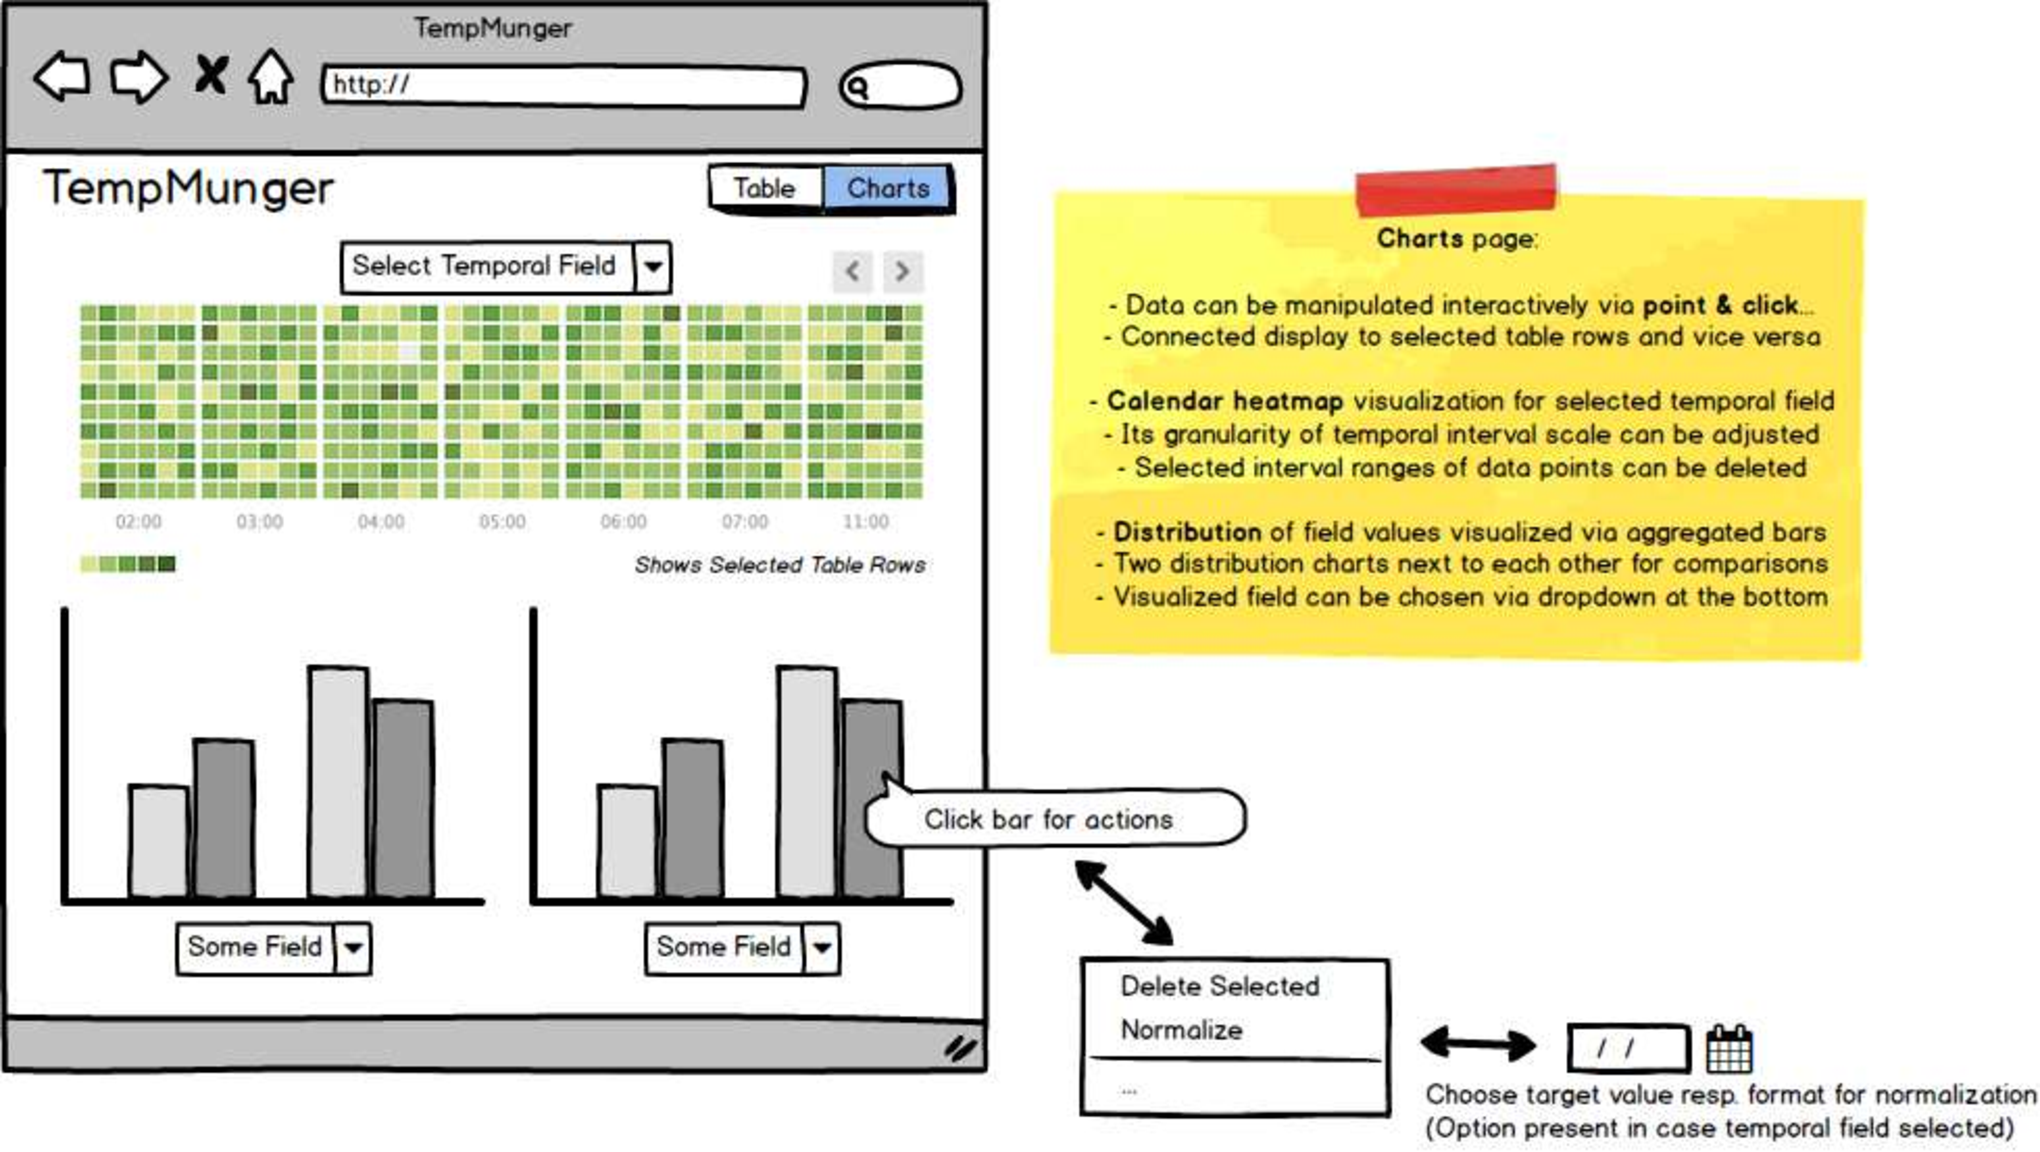
\includegraphics[width=1.0\textwidth]{../thesis/figures/design/mockup-6_cmyk}
          \caption{UI mockup of the charts page including calendar heatmap visualization.}
          \label{fig:mockup-6}
        \end{figure}

        \begin{figure}[h]
          \centering
          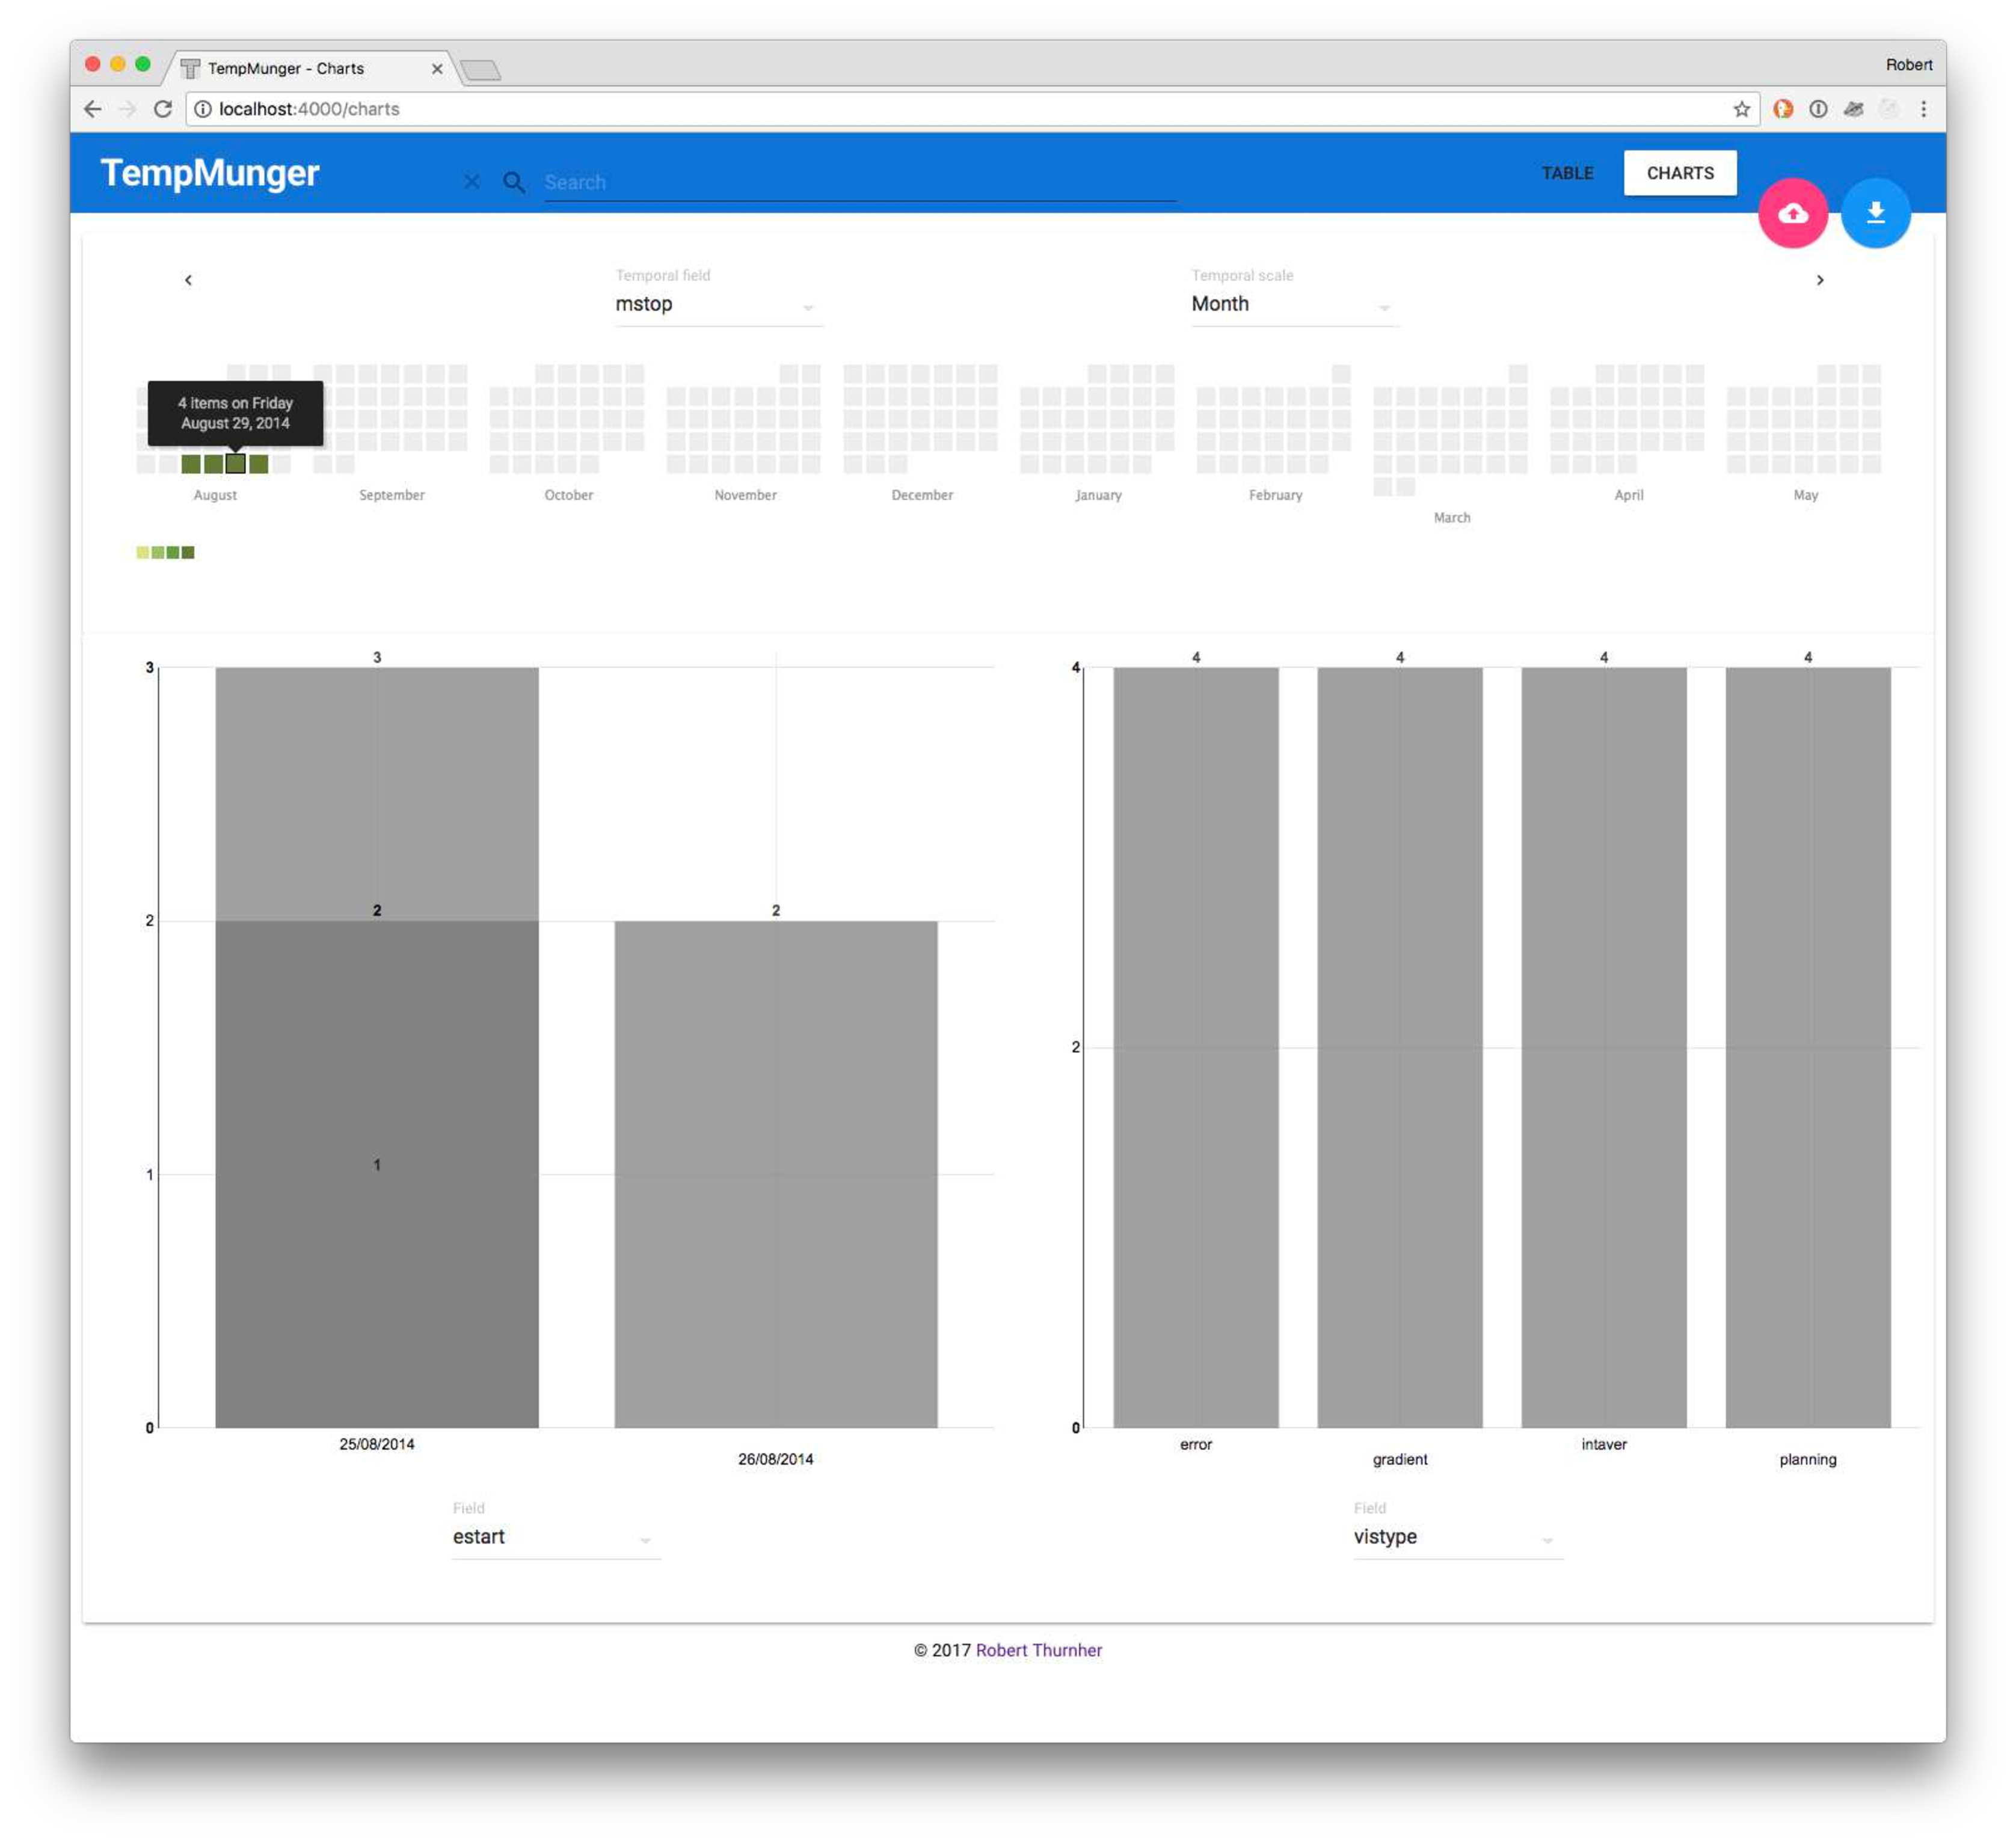
\includegraphics[width=1.0\textwidth]{../thesis/figures/implementation/screenshot-charts-page_cmyk}
          \caption{Screenshot of the resulting charts page, offering visual overview.}
          \label{fig:screenshot-charts-page}
        \end{figure}
      \end{block}

      \begin{block}{References}
        \bibliographystyle{unsrt}
        \bibliography{../thesis/references}
      \end{block}
    \end{column}
    % ---------------------------------------------------------%
    % end the column
  \end{columns}

\end{frame}

\end{document}

%%% Local Variables:
%%% TeX-PDF-mode: t
%%% TeX-debug-bad-boxes: t
%%% TeX-master: t
%%% TeX-parse-self: t
%%% TeX-auto-save: t
%%% reftex-plug-into-AUCTeX: t
%%% End:
